
\documentclass[preview,convert,convert={outext=.png,command=\unexpanded{pdftocairo -r 600 -png \infile}}]{standalone}
\usepackage{graphicx}
\usepackage{subfig}
\graphicspath{{/home/ming/academic/tools/latex2word/tests/zh/figures}}
\usepackage{xeCJK}
\begin{document}
\thispagestyle{empty}
\begin{figure}[htbp]
    \centering
    \subfloat[] {
        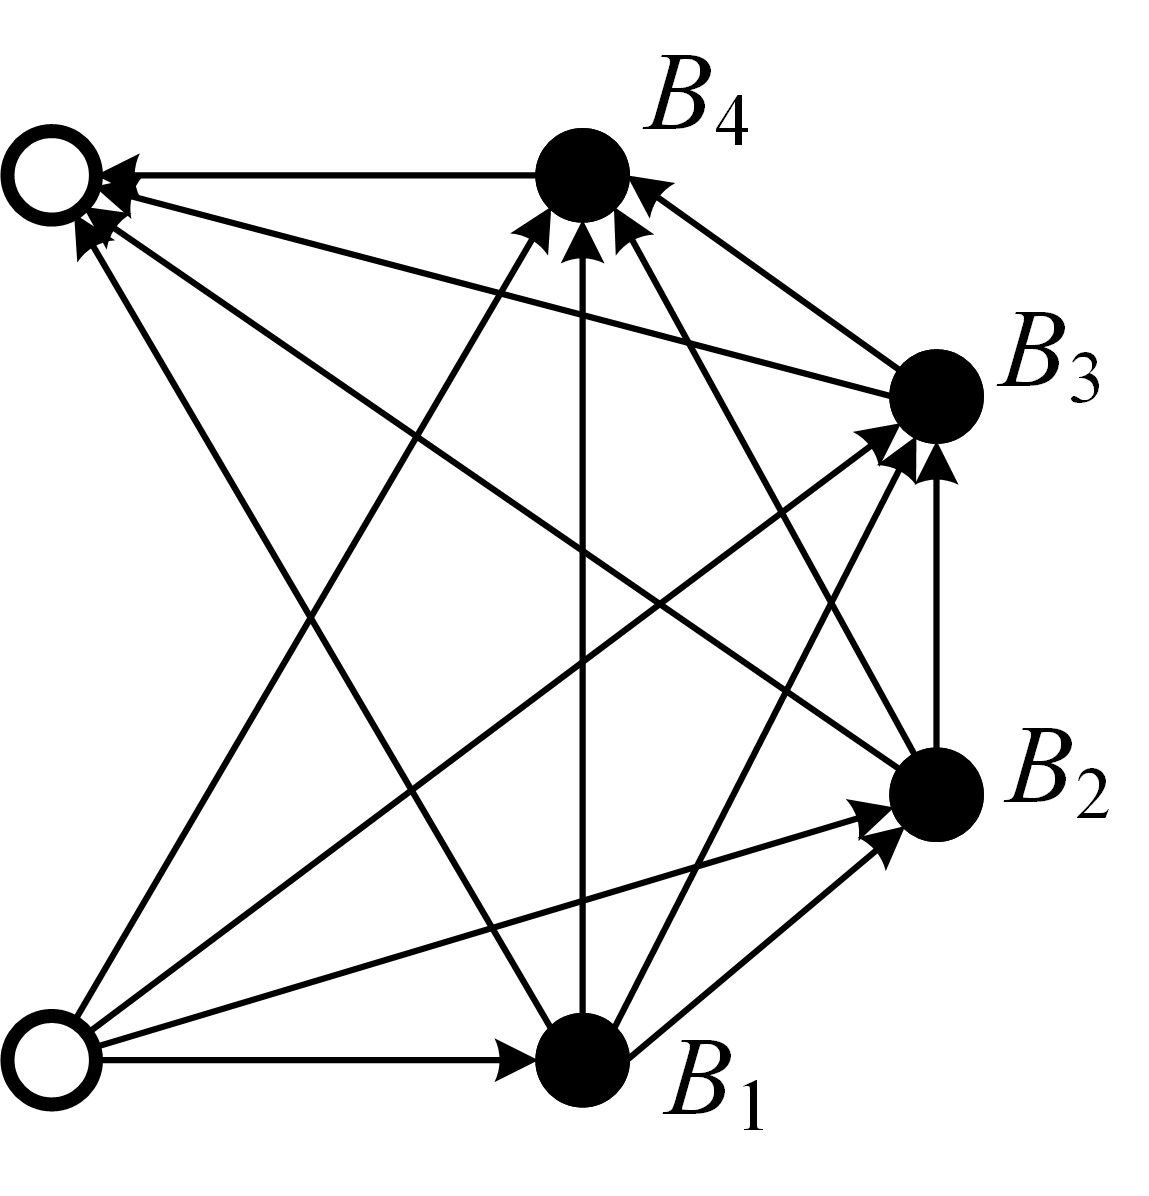
\includegraphics[width=0.31\linewidth]{direct-graph-he.png}
    }\label{fig:direct-graph-he}
    \subfloat[] {
        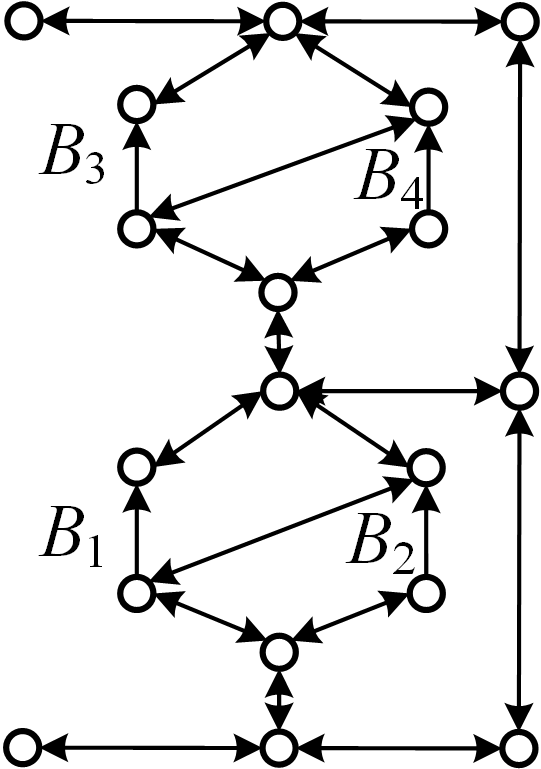
\includegraphics[width=0.23\linewidth]{direct-graph-xu.png}
    }\label{fig:direct-graph-xu}
    \subfloat[] {
        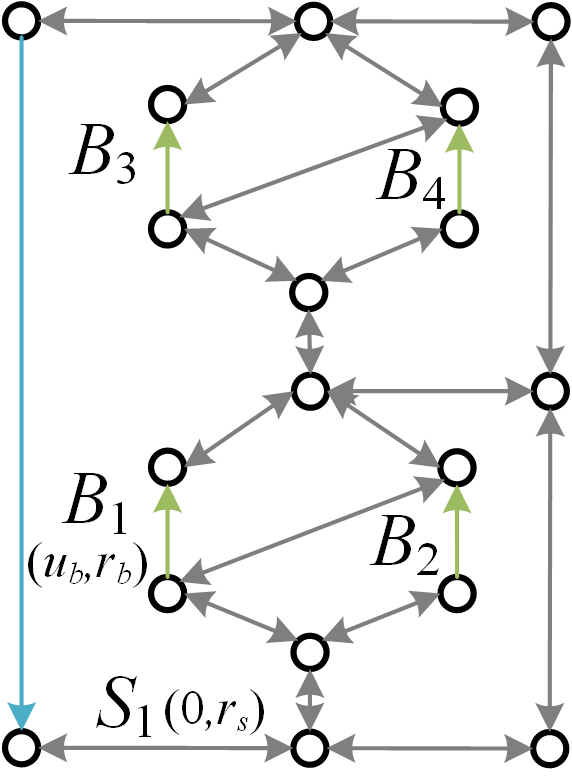
\includegraphics[width=0.24\linewidth]{direct-graph-my.png}
    }\label{fig:direct-graph-my}
    \\
    \subfloat[] {
        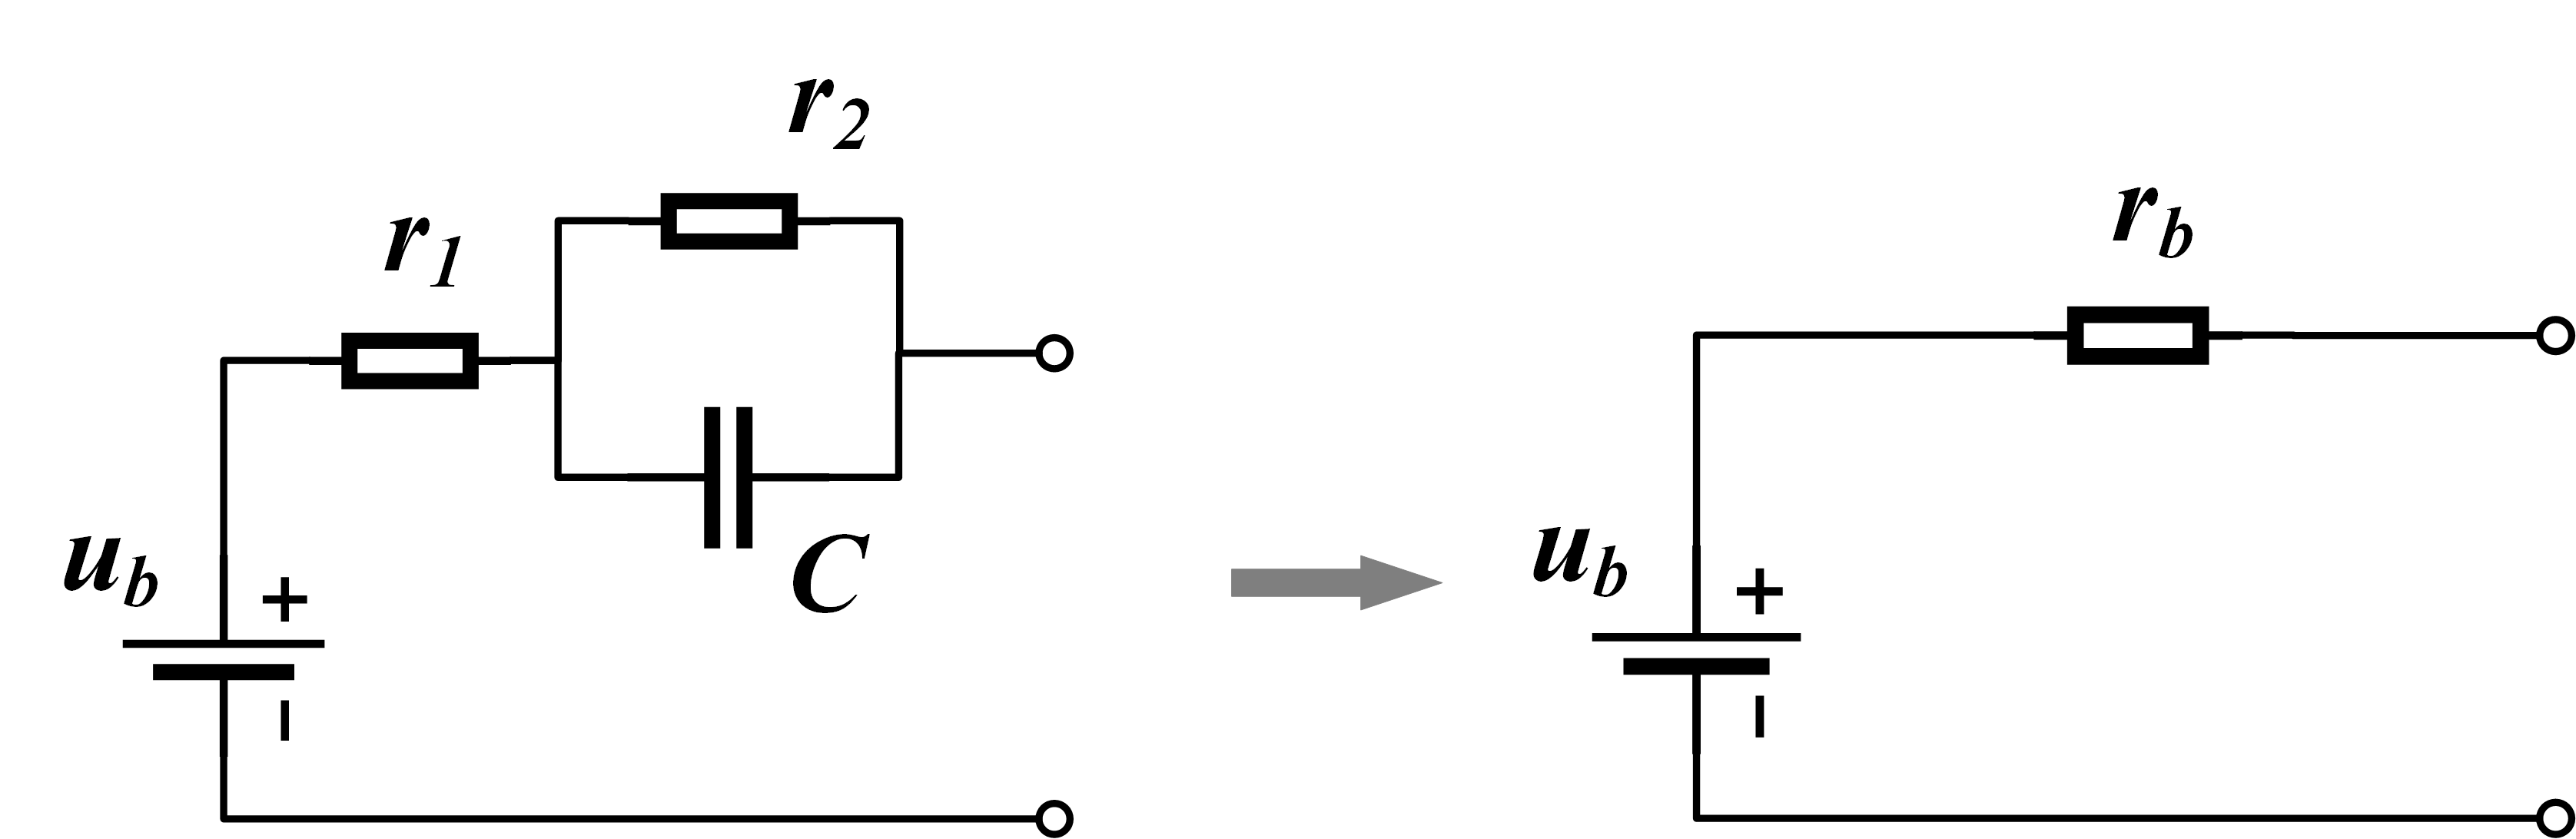
\includegraphics[width=0.8\linewidth]{battery_simple.png}
    }\label{fig:battery-simple}
    %\caption{
%        定向图模型: (a) He等人的工作 \cite{heExploringAdaptiveReconfiguration2013},(b) 我们之前的工作,(c) 本文提出的改进模型。 (d) 本方法中的电池等效电路图。
%    }
    \label{fig:model}
\end{figure}
\end{document}
